\appendix
\section{Basic Bricks of the Trade}
This appendix is written here for the completeness of the proof of lemma \ref{lemma3}.
\par
In homotopy theory every map $f: A \rightarrow B$ from a space $A$ to a pathconnected space $B$ may be viewed as either an inclusion or a fibering. We can see this as follows.
\subsection{Inclusion} 
\label{inc}
Applying the telescoping idea just once, we construct the mapping cylinder of $f$:

\begin{figure}[h!]
\centering
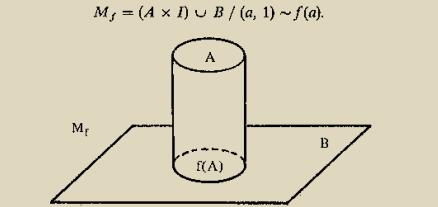
\includegraphics[scale=1]{mappingcylinder.jpg}
\caption{mapping cylinder}
\label{UN}
\end{figure}
It is clear that the mapping cyinder $M_{f}$ has the same homotopy type as $B$ and that $A$ is included in $M_{f}$. Indeed the following diagram is commutative:
$$
\xymatrix{
A \ar[d]^{id} \ar[r]^f &B\ar@{^{(}->}[d]^{\text{homotopy equivalence}}\\
A\ar@{^{(}->}[r] & M_f}
$$
\subsection{Fibering}
Let $f: A \rightarrow B$ be any map, with $B$ path connected. By section \ref{inc} we may assume that $f$ is an inclusion, i.e., $A$ is a subspace of $B$. Define
$L$ to be the space of all paths in $B$ with initial point in $A$. By shrinking every path to its initial point, we get a homotopy equivalence
\[
L \simeq A
\]
On the other hand by projecting every path to its endpoint, we get a fibering
\[
\begin{array}{c}
\Omega_{*}^{A}-L_{*} A \\
\downarrow_{ } \\
B
\end{array}
\]
$$\xymatrix{
\Omega_{*}^{A}\ar[r]& L \ar[d]\\
&B
}$$
Whose fiber is $\Omega_{*}^{A},$ the space of all paths from a point $*$ in $B$ to $A .$ So up to homotopy equivalence, $f: A \rightarrow B$ is a fibering.